%
%
%% Enter Figures and Tables here:
%
% DO NOT USE \psfrag or \subfigure commands.
%
% Figure captions go below the figure.
% Table titles go above tables; all other caption information
%  should be placed in footnotes below the table.
%
%----------------
% BEGIN FIGUREs
%

\clearpage
\begin{figure}[t]
  \begin{center}
    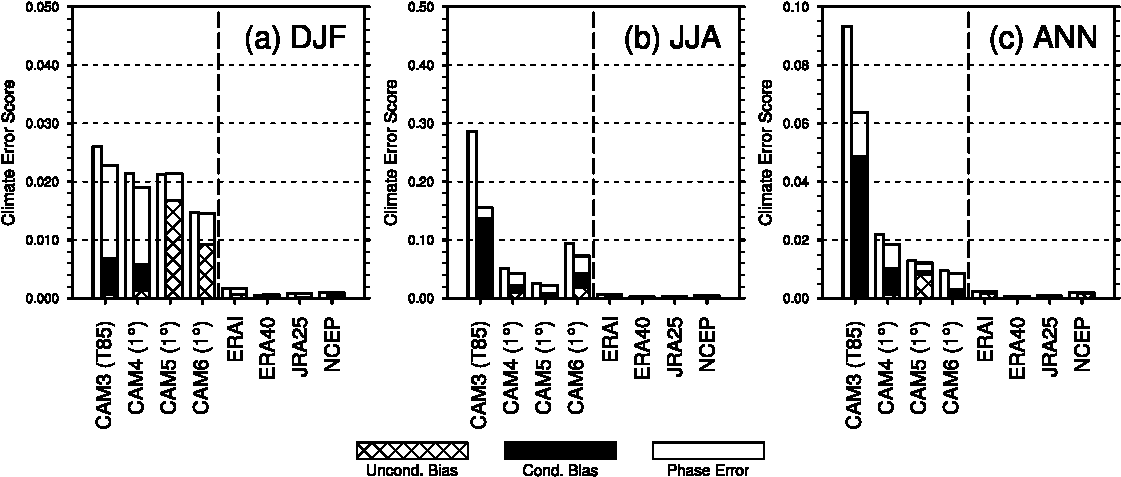
\includegraphics[width=1\textwidth,angle=0.]{./figs/f_skill_score.pdf}
 \end{center}
  \caption {Seasonal climatology of contributions to the Normalized Mean Square Error (NMSE) over the northern hemisphere (30$^\circ$ N-90$^\circ$ N) for CAM releases between CAM3 and CAM6. Individual contributions are the unconditional bias (hatched), conditional bias (solid) and phase error (unfilled). The narrow unfilled bar for each model is the scaled variance ratio (SVR). The model is compared to the ECMWF (ERA15) reanalysis. Contemporary analysis (JRA25/NCEP/ERA40 and ERA-interim) biases compared top ECMWF are also shown.} 
\label{f_skill_score}
\end{figure} 
%%
\clearpage
\begin{figure}[t]
  \begin{center}
    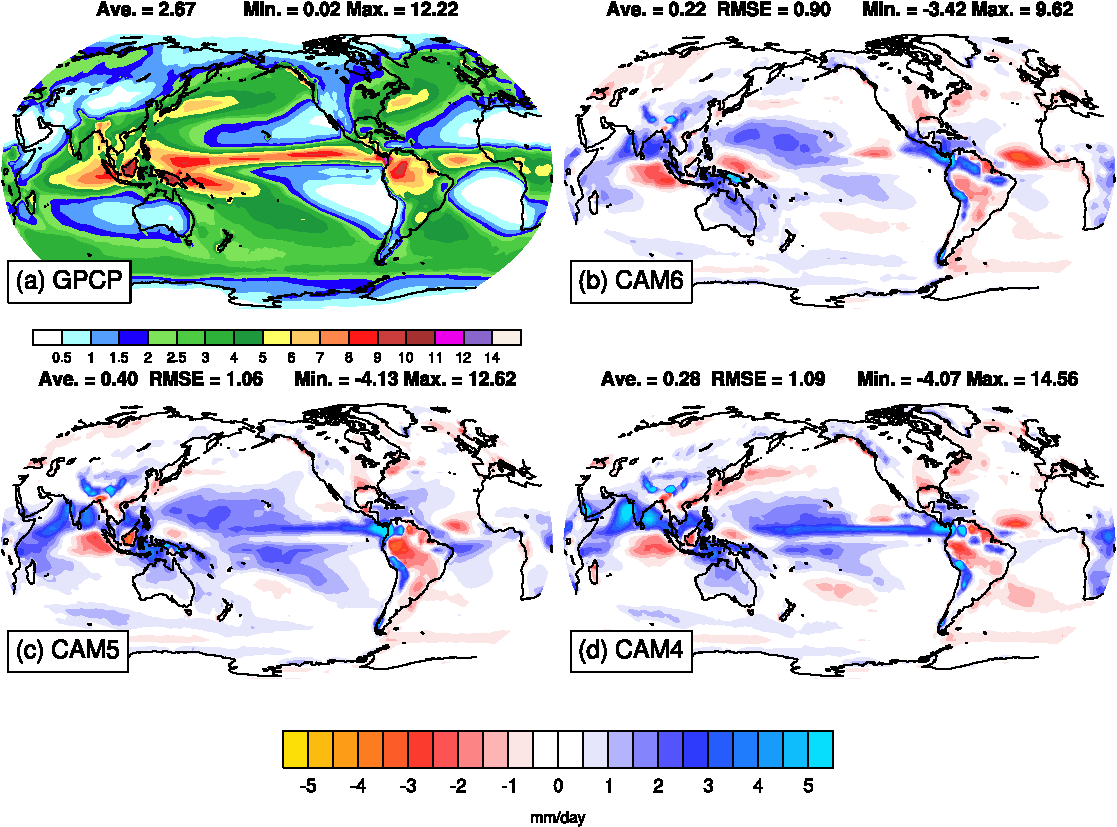
\includegraphics[width=1.\textwidth,angle=90.]{./figs/f_PRECT_2D_CAM456.pdf}
  \end{center}
  \caption{Climatology of annual precipitation (mm/day) for (a) Observations (GPCP, 19XX-20XX), and its biases for (a) CAM4 (b) CAM5  through CAM6 AMIP simulations for the period 1979-2005. Hatched areas are where wet biases exceed 100\% of observed and vertical line regions are where dry biases are greater than 25\% of observed.}
\label{f_PRECT_2D_CAM456}
\end{figure}

%%
\clearpage
\begin{figure}[t]
  \begin{center}
    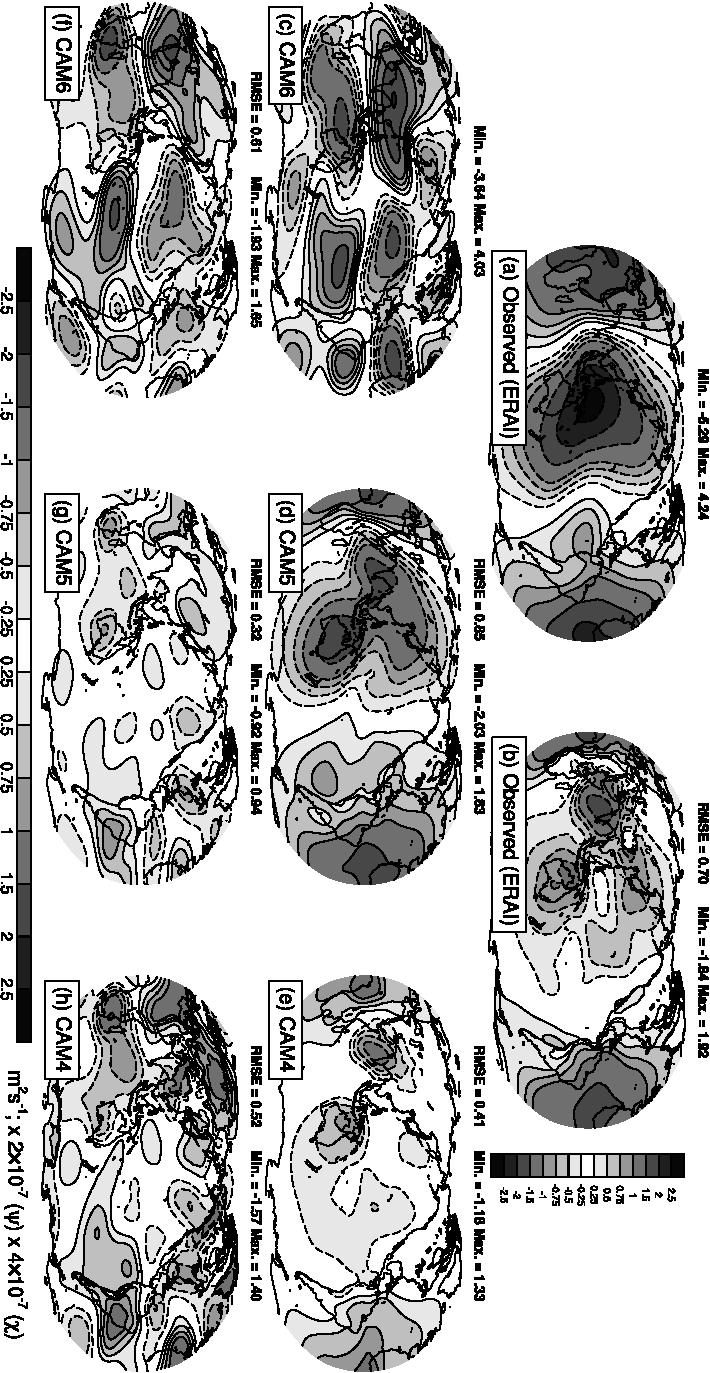
\includegraphics[width=0.55\textwidth,angle=90.]{./figs/f_PSICHI_2D_ANN_CAM456.pdf}
  \end{center}
  \caption{Climatology of annual precipitation (mm/day) for (a) Observations (GPCP, 19XX-20XX), and its biases for (a) CAM4 (b) CAM5  through CAM6 AMIP simulations for the period 1979-2005. Hatched areas are where wet biases exceed 100\% of observed and vertical line regions are where dry biases are greater than 25\% of observed.}
\label{f_PSICHI_2D_CAM456}
\end{figure}

%%
\clearpage
\begin{figure}[t]
  \begin{center}
    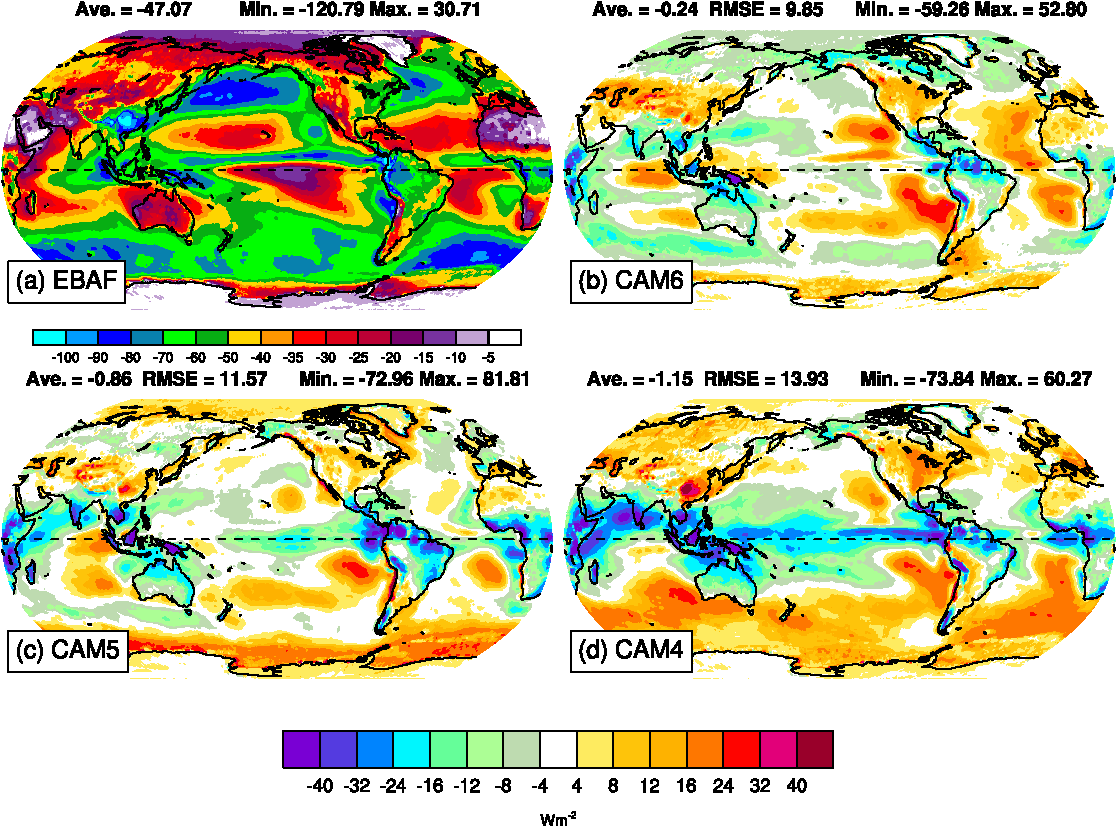
\includegraphics[width=1.\textwidth,angle=0.]{./figs/f_SWCF_2D_CAM456_ANN.pdf}
  \end{center}
  \caption{Climatology of annual  (mm/day) for (a) Observations (GPCP, 19XX-20XX), and its biases for (a) CAM4 (b) CAM5  through CAM6 AMIP simulations for the period 1979-2005. Hatched areas are where wet biases exceed 100\% of observed and vertical line regions are where dry biases are greater than 25\% of observed.}
\label{f_PRECT_2D_CAM456}
\end{figure}
%%
\clearpage
\begin{figure}[t]
%  \begin{center}
    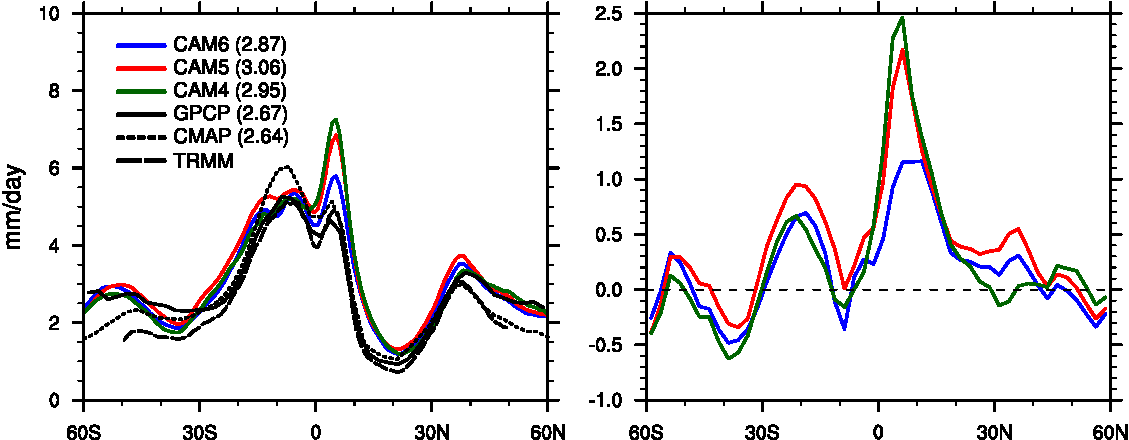
\includegraphics[width=1.\textwidth,angle=0.]{./figs/f_PRECT_1D_DJF_CAM456.pdf}
%  \end{center}
  \caption{Climatology of annual precipitation (mm/day) for (a) Observations (GPCP, 19XX-20XX), and its biases for (a) CAM4 (b) CAM5  through CAM6 AMIP simulations for the period 1979-2005} 
\label{f_PRECT_1D_DJF_CAM456}
\end{figure} 
%%
\clearpage
\begin{figure}[t]
  \begin{center}
    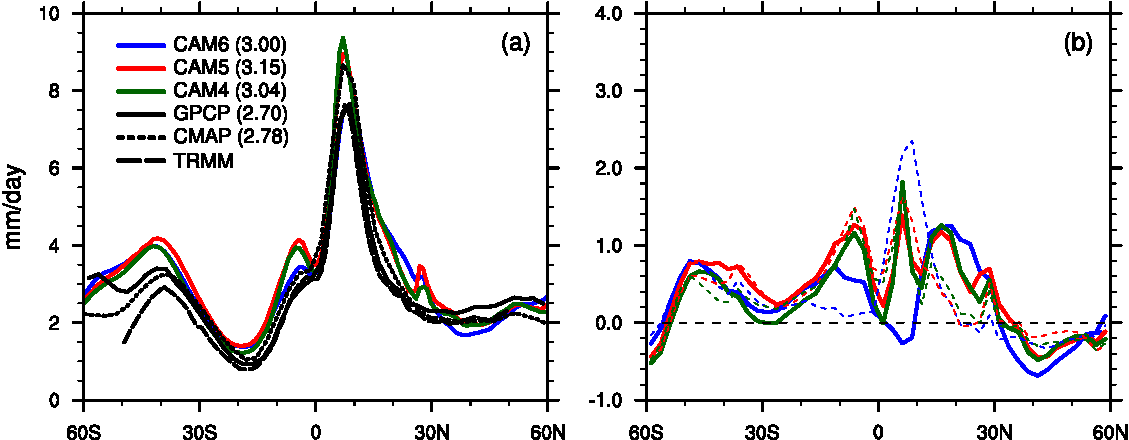
\includegraphics[width=1.\textwidth,angle=0.]{./figs/f_PRECT_1D_JJA_CAM456.pdf}
  \end{center}
  \caption{Climatology of annual precipitation (mm/day) for (a) Observations (GPCP, 19XX-20XX), and its biases for (a) CAM4 (b) CAM5  through CAM6 AMIP simulations for the period 1979-2005} 
\label{f_PRECT_1D_JJA_CAM456}
\end{figure} 


%%
\clearpage
\begin{figure}[t]
%  \begin{center}
    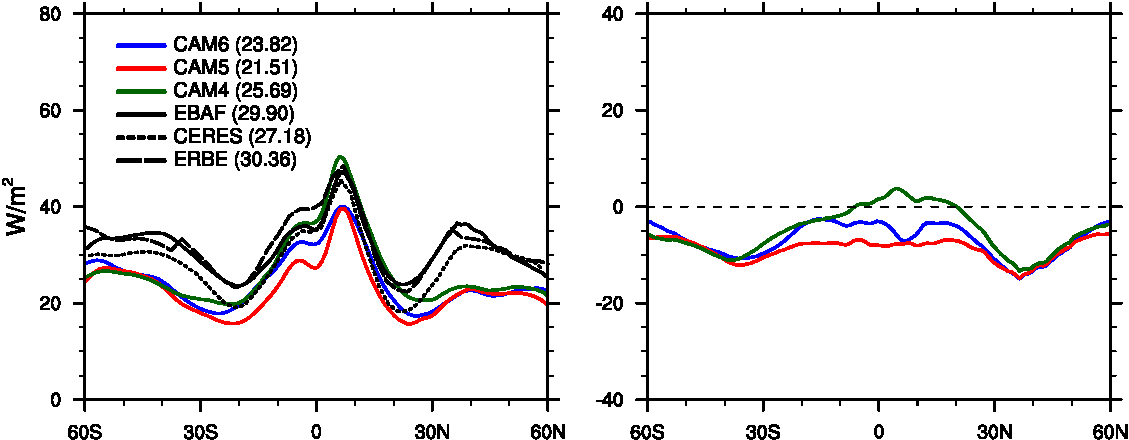
\includegraphics[width=1.\textwidth,angle=0.]{./figs/f_LWCF_1D_ANN_CAM456.pdf}
%  \end{center}
  \caption{Climatology of annual precipitation (mm/day) for (a) Observations (GPCP, 19XX-20XX), and its biases for (a) CAM4 (b) CAM5  through CAM6 AMIP simulations for the period 1979-2005} 
\label{f_LWCF_1D_ANN_CAM456}
\end{figure} 

%%
\clearpage
\begin{figure}[t]
  \begin{center}
    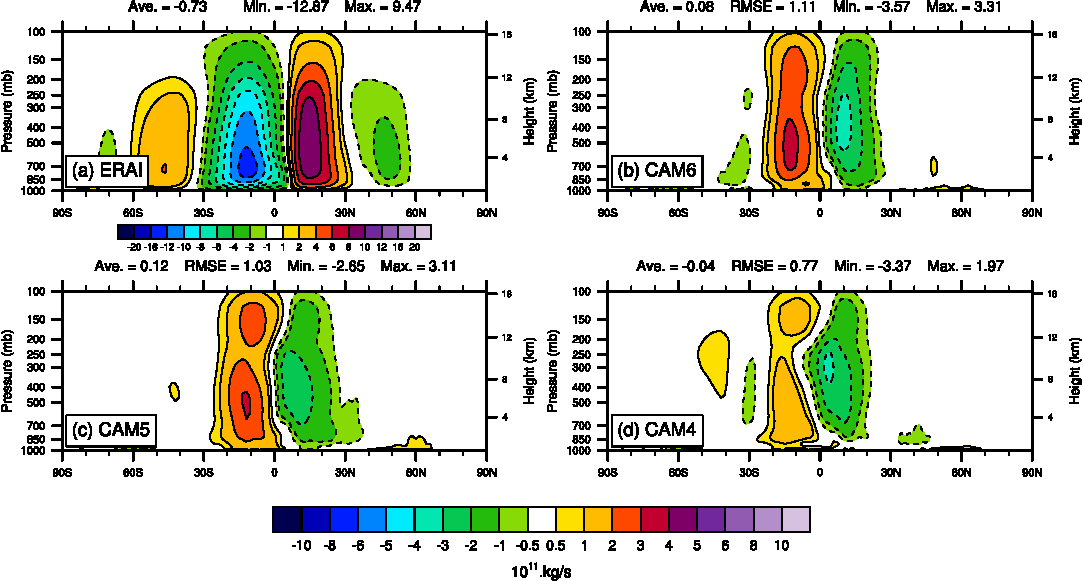
\includegraphics[width=1.1\textwidth,angle=0.]{./figs/f_MMC_2D_ANN_CAM456.pdf}
  \end{center}
  \caption{Climatology of annual mean meridional circulation (units) for (a) Observations (ERA-interim 19XX-20XX) and biases for (b) CAM6, (c) CAM5 and (d) CAM4.} 
\label{f_MMC_2D_ANN_CAM456}
\end{figure} 


%%
\clearpage
\begin{figure}[t]
%  \begin{center}
    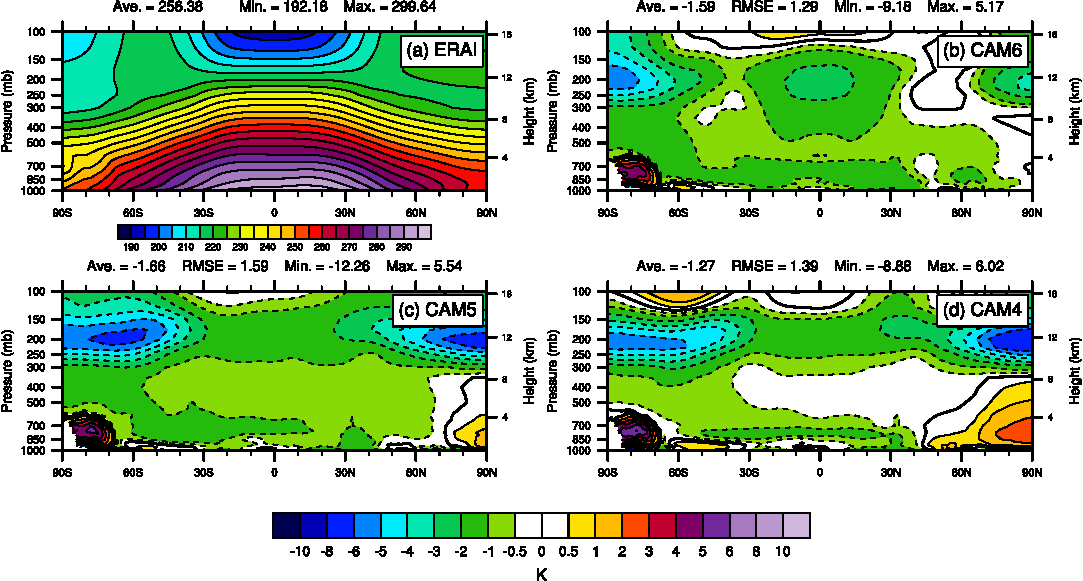
\includegraphics[width=1.\textwidth,angle=0.]{./figs/f_T_2D_ANN_CAM456.pdf}
%  \end{center}
  \caption{Climatology of annual mean temperature (K) for (a) Observations (GPCP, 19XX-20XX), and its biases for (a) CAM4 (b) CAM5  through CAM6 AMIP simulations for the period 1979-2005} 
\label{f_T_2D_ANN_CAM456}
\end{figure} 


%%
\clearpage
\begin{figure}[t]
%  \begin{center}
    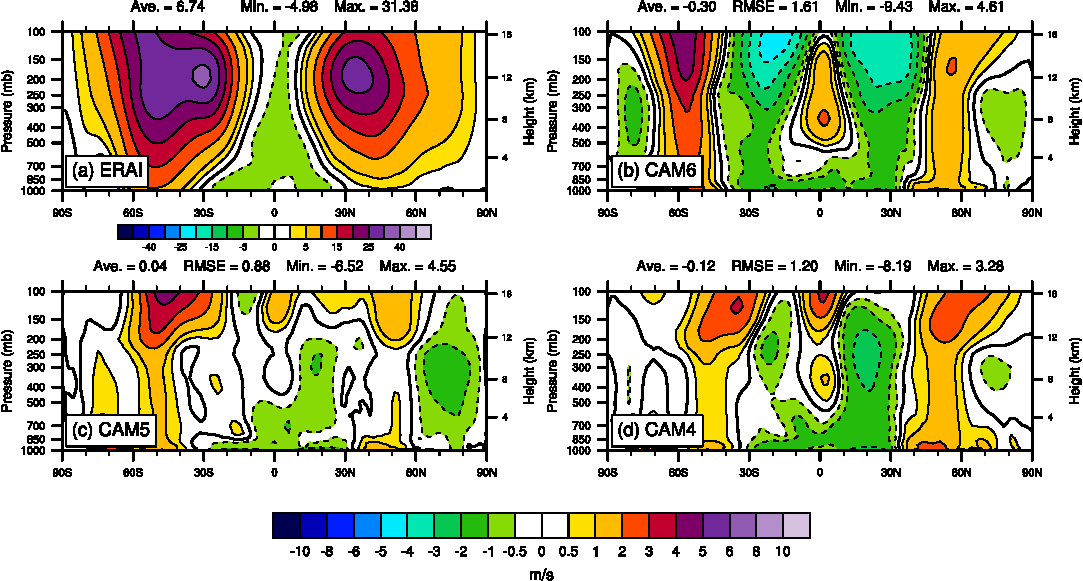
\includegraphics[width=1.\textwidth,angle=0.]{./figs/f_U_2D_ANN_CAM456.pdf}
%  \end{centerf_VPROF_NITCZ.pdf}
  \caption{Climatology of annual mean zonal wind) Observations (GPCP, 19XX-20XX), and its biases for (a) CAM4 (b) CAM5  through CAM6 AMIP simulations for the period 1979-2005} 
\label{f_U_2D_ANN_CAM456}
\end{figure} 



%%
\clearpage
\begin{figure}[t]
  \begin{center}
    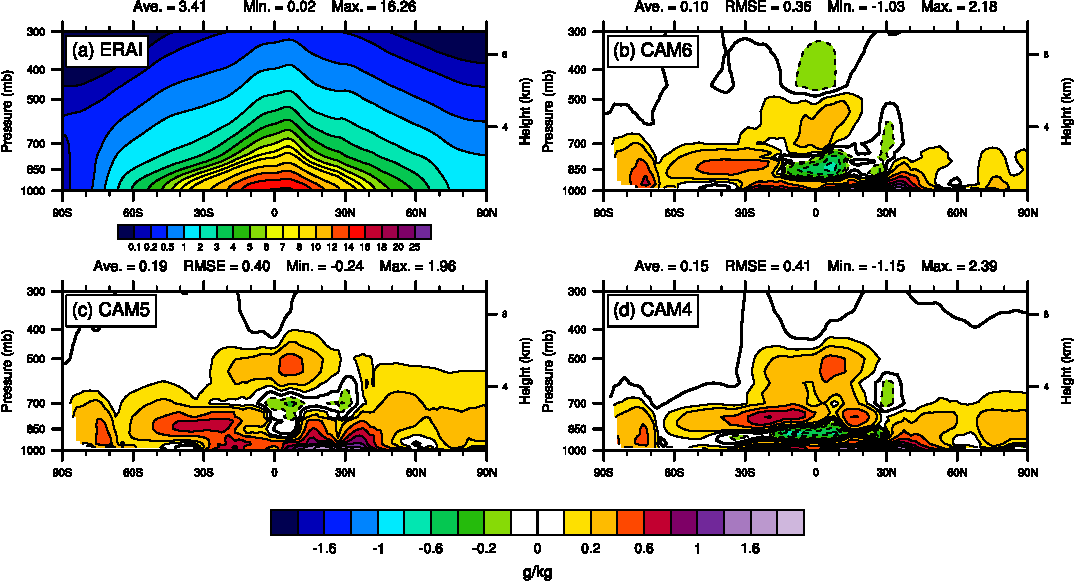
\includegraphics[width=1.\textwidth,angle=0.]{./figs/f_MERRA_Q_latp_diff_ANN.pdf}
  \end{center}
  \caption{Climatology of annual precipitation (mm/day) for (a) Observations (GPCP, 19XX-20XX), and its biases for (a) CAM4 (b) CAM5  through CAM6 AMIP simulations for the period 1979-2005} 
\label{MERRA_Q_latp_diff_ANN}
\end{figure} 



%%%%%%%%%%%%%%%%%%%%%%%%%%%
%%%%%%% TENDENCIES %%%%%%%%
%%%%%%%%%%%%%%%%%%%%%%%%%%%

%%
\clearpage
\begin{figure}[t]
  \begin{center}
    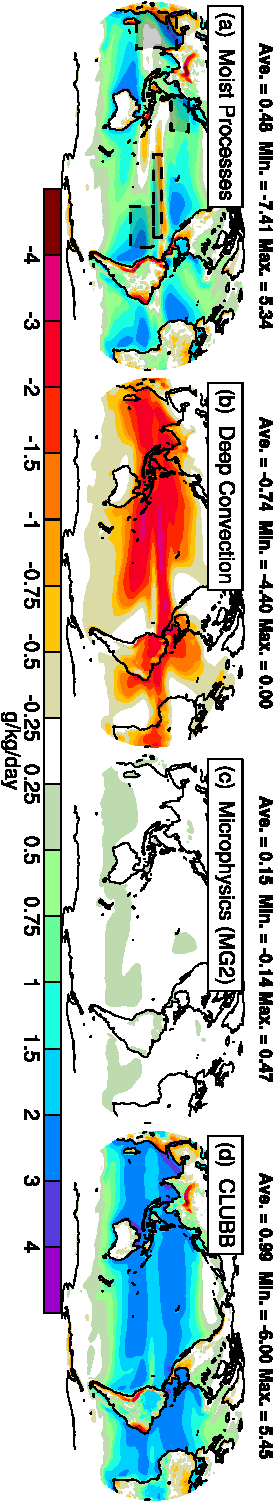
\includegraphics[width=0.2\textwidth,angle=90.]{./figs/f_DQDT_PBL_2D_CAM6_ANN.pdf}
  \end{center}
  \caption{Annual climatology of CAM6 tendencies of humidity from the primary physical process parameterizations vertically averaged between the surface and 800 hPa.} 
\label{f_DQDT_PBL_2D_CAM6_ANN}
\end{figure} 

%%
\clearpage
\begin{figure}[t]
  \begin{center}
    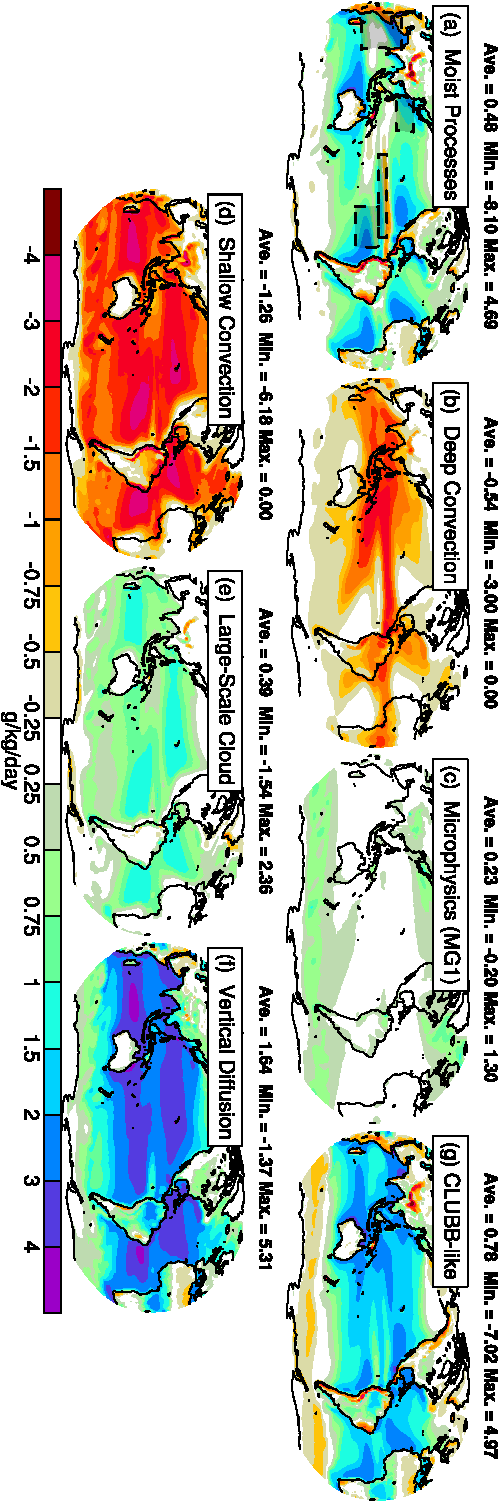
\includegraphics[width=0.4\textwidth,angle=90.]{./figs/f_DQDT_PBL_2D_CAM5_ANN.pdf}
  \end{center}
  \caption{Annual climatology of CAM5 tendencies of humidity from the primary physical process parameterizations vertically averaged between the surface and 800 hPa.} 
\label{f_DQDT_PBL_2D_CAM5_ANN}
\end{figure} 



%%
\clearpage
\begin{figure}[t]
  \begin{center}
    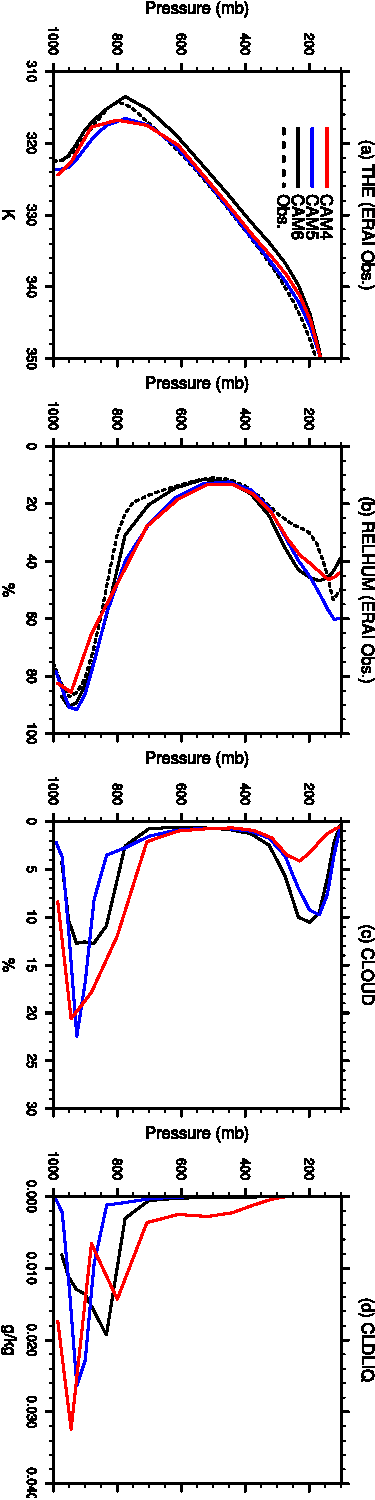
\includegraphics[width=0.24\textwidth,angle=90.]{./figs/f_VPROF_EPAC_JJA.pdf}
  \end{center}
  \caption{Vertical profiles of JJA climatology for CAM4, CAM5, CAM6 and observations of (a) equivalent potential temperature (THE, K), relative humidity (RELHUM, \%), total cloud fraction (CLOUD, \%) and (grid box averae cloud liquid (CLDLIQ, \g/kg). Data is averaged over the "East Pacific" region.} 
\label{f_VPROF_NITCZ._JJA}
\end{figure} 

%%
\clearpage
\begin{figure}[t]
  \begin{center}
    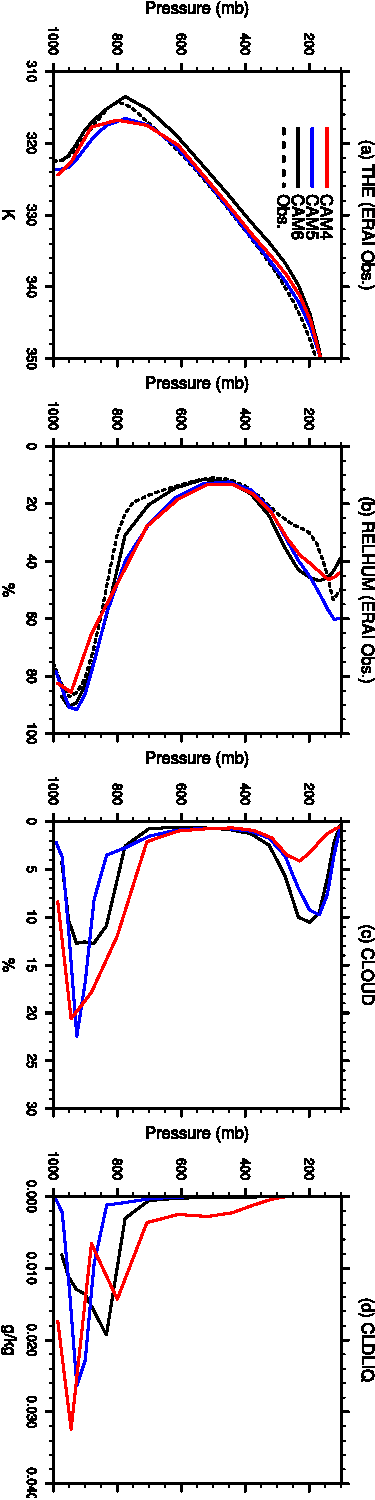
\includegraphics[width=0.24\textwidth,angle=90.]{./figs/f_VPROF_EPAC_JJA.pdf}
  \end{center}
  \caption{Vertical profiles of JJA climatology for CAM4, CAM5, CAM6 and observations of (a) equivalent potential temperature (THE, K), relative humidity (RELHUM, \%), total cloud fraction (CLOUD, \%) and (grid box averae cloud liquid (CLDLIQ, \g/kg). Data is averaged over the "East Pacific" region.} 
\label{f_VPROF_NITCZ._JJA}
\end{figure} 

%%
\clearpage
\begin{figure}[t]
  \begin{center}
    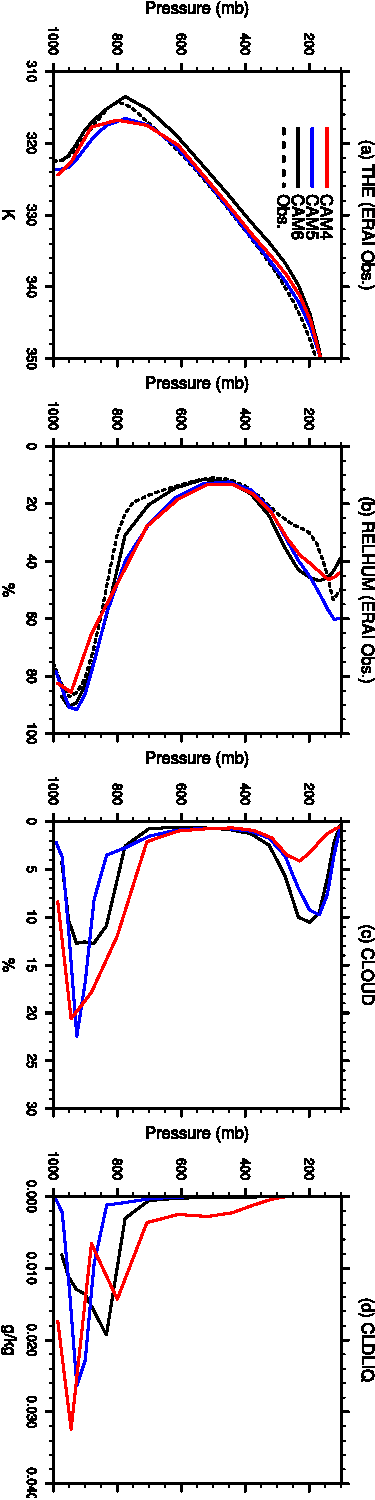
\includegraphics[width=0.24\textwidth,angle=90.]{./figs/f_VPROF_EPAC_JJA.pdf}
  \end{center}
  \caption{Vertical profiles of JJA climatology for CAM4, CAM5, CAM6 and observations of (a) equivalent potential temperature (THE, K), relative humidity (RELHUM, \%), total cloud fraction (CLOUD, \%) and (grid box averae cloud liquid (CLDLIQ, \g/kg). Data is averaged over the "East Pacific" region.} 
\label{f_VPROF_NITCZ._JJA}
\end{figure} 


